\chapter{Introduction}
\label{chap1:introduction}

In recent years, few areas of research have enjoyed similar manifestations of interest and enthusiasm as \ac{DL}. Staggering amounts of progress have been made, culminating in models that can do seemingly everything: image classification, object detection, image synthesis, amongst many others. As the remainder of this document will make clear, \ac{DL} models (and other \ac{ML} techniques) can be used in creative pipelines, incorporating each architecture's strengths. Such wide availability of solutions proves how accessible the field has become.\\

Fortunately for the research community, within the field of \ac{DL}, there is still some ground to cover in emerging areas. Explainability is one of those areas, with active lines of research. Most of the techniques found in literature find their way into existing systems due to a need for explanations. Not by design, but by requirement. Usually, this need comes after the system's deployment, as a quick fix. We argue that this mindset is no longer realistic, especially in areas where decisions need to be accurate and frequently audited. Even if the system's environment does not require intensive validation, ensuring some degree of explainability should always be desirable (it could, perhaps, be considered a "good practice").\\

Based on what was stated above, in this work we are interested in incorporating explainable components into a system, that given a pair of images from the periocular region, is capable of delivering a twofold output: a binary decision ("yes" or "no"), supported by a pleasing (and visual) explanation. The former is similar to a classical approach, while the latter serves the emerging need for decision validation.

\section{Motivations and Objectives}
\label{sec:chap1_motivations_and_objectives}
The present document aims at presenting a view of the state of \ac{ML} Explainability, as well as, describing ways to merge such techniques with standard \ac{DL} methods. By compiling several approaches with adequate descriptions, we hope to clarify the concepts behind explainable \ac{AI} and how it actually works. Such knowledge is becoming increasingly more valuable as \ac{ML} systems find their way into real world scenarios. \\

Regarding the specific goals of this work, we aim at developing an integrated framework that performs periocular recognition and automatically produces easy to understand explanations. By doing so, we are not only accomplishing a useful task but also bridging the gap between our system's reasoning and the users that may end up using it.

\section{Document Organisation}
\label{sec:chap1_document_organisation}
In order to provide an intuitive reading experience, this document is divided according to the following chapters: 

\begin{enumerate}
    \item \textbf{Introduction} - provides a general overview of this work's motivations and objectives, as well as, the structure by which this document is organised.
    \item \textbf{Related Work} - presents an extensive look at widely used algorithms and techniques in the fields of interest.
    \item \textbf{Proposed Methods} - showcases the methods and intuitions developed to tackle the problem at hand.
    \item \textbf{Results and Discussion} - contains the experiments performed to validate the proposed methods, with accompanying results and discussions.
    \item \textbf{Conclusions and Further Work} - concludes the present document with both a review of the work and its potential improvements in the future.
\end{enumerate}

\section{Dissertation Outline}
\label{sec:chap1_dissertation_outline}

In order to perceive the workflow that this dissertation encompassed, Fig. \ref{fig:gantt_diagram} depicts a simple Gantt diagram with the tasks performed and how long they took to complete. Naturally, the work started by devoting several months towards research on the topics of interest: Biometric Recognition, \ac{DL} and \ac{ML} Explainability. Then, this foundation was put to use during the development of both proposed methods (while the first one consumed a lengthier, uninterrupted time span, the second method required additional research for adequate \ac{DL} models). Finally, the results conveyed by our experiments were analysed so as to better understand if the original goal had been achieved:\\

\begin{figure}[h]
\centering
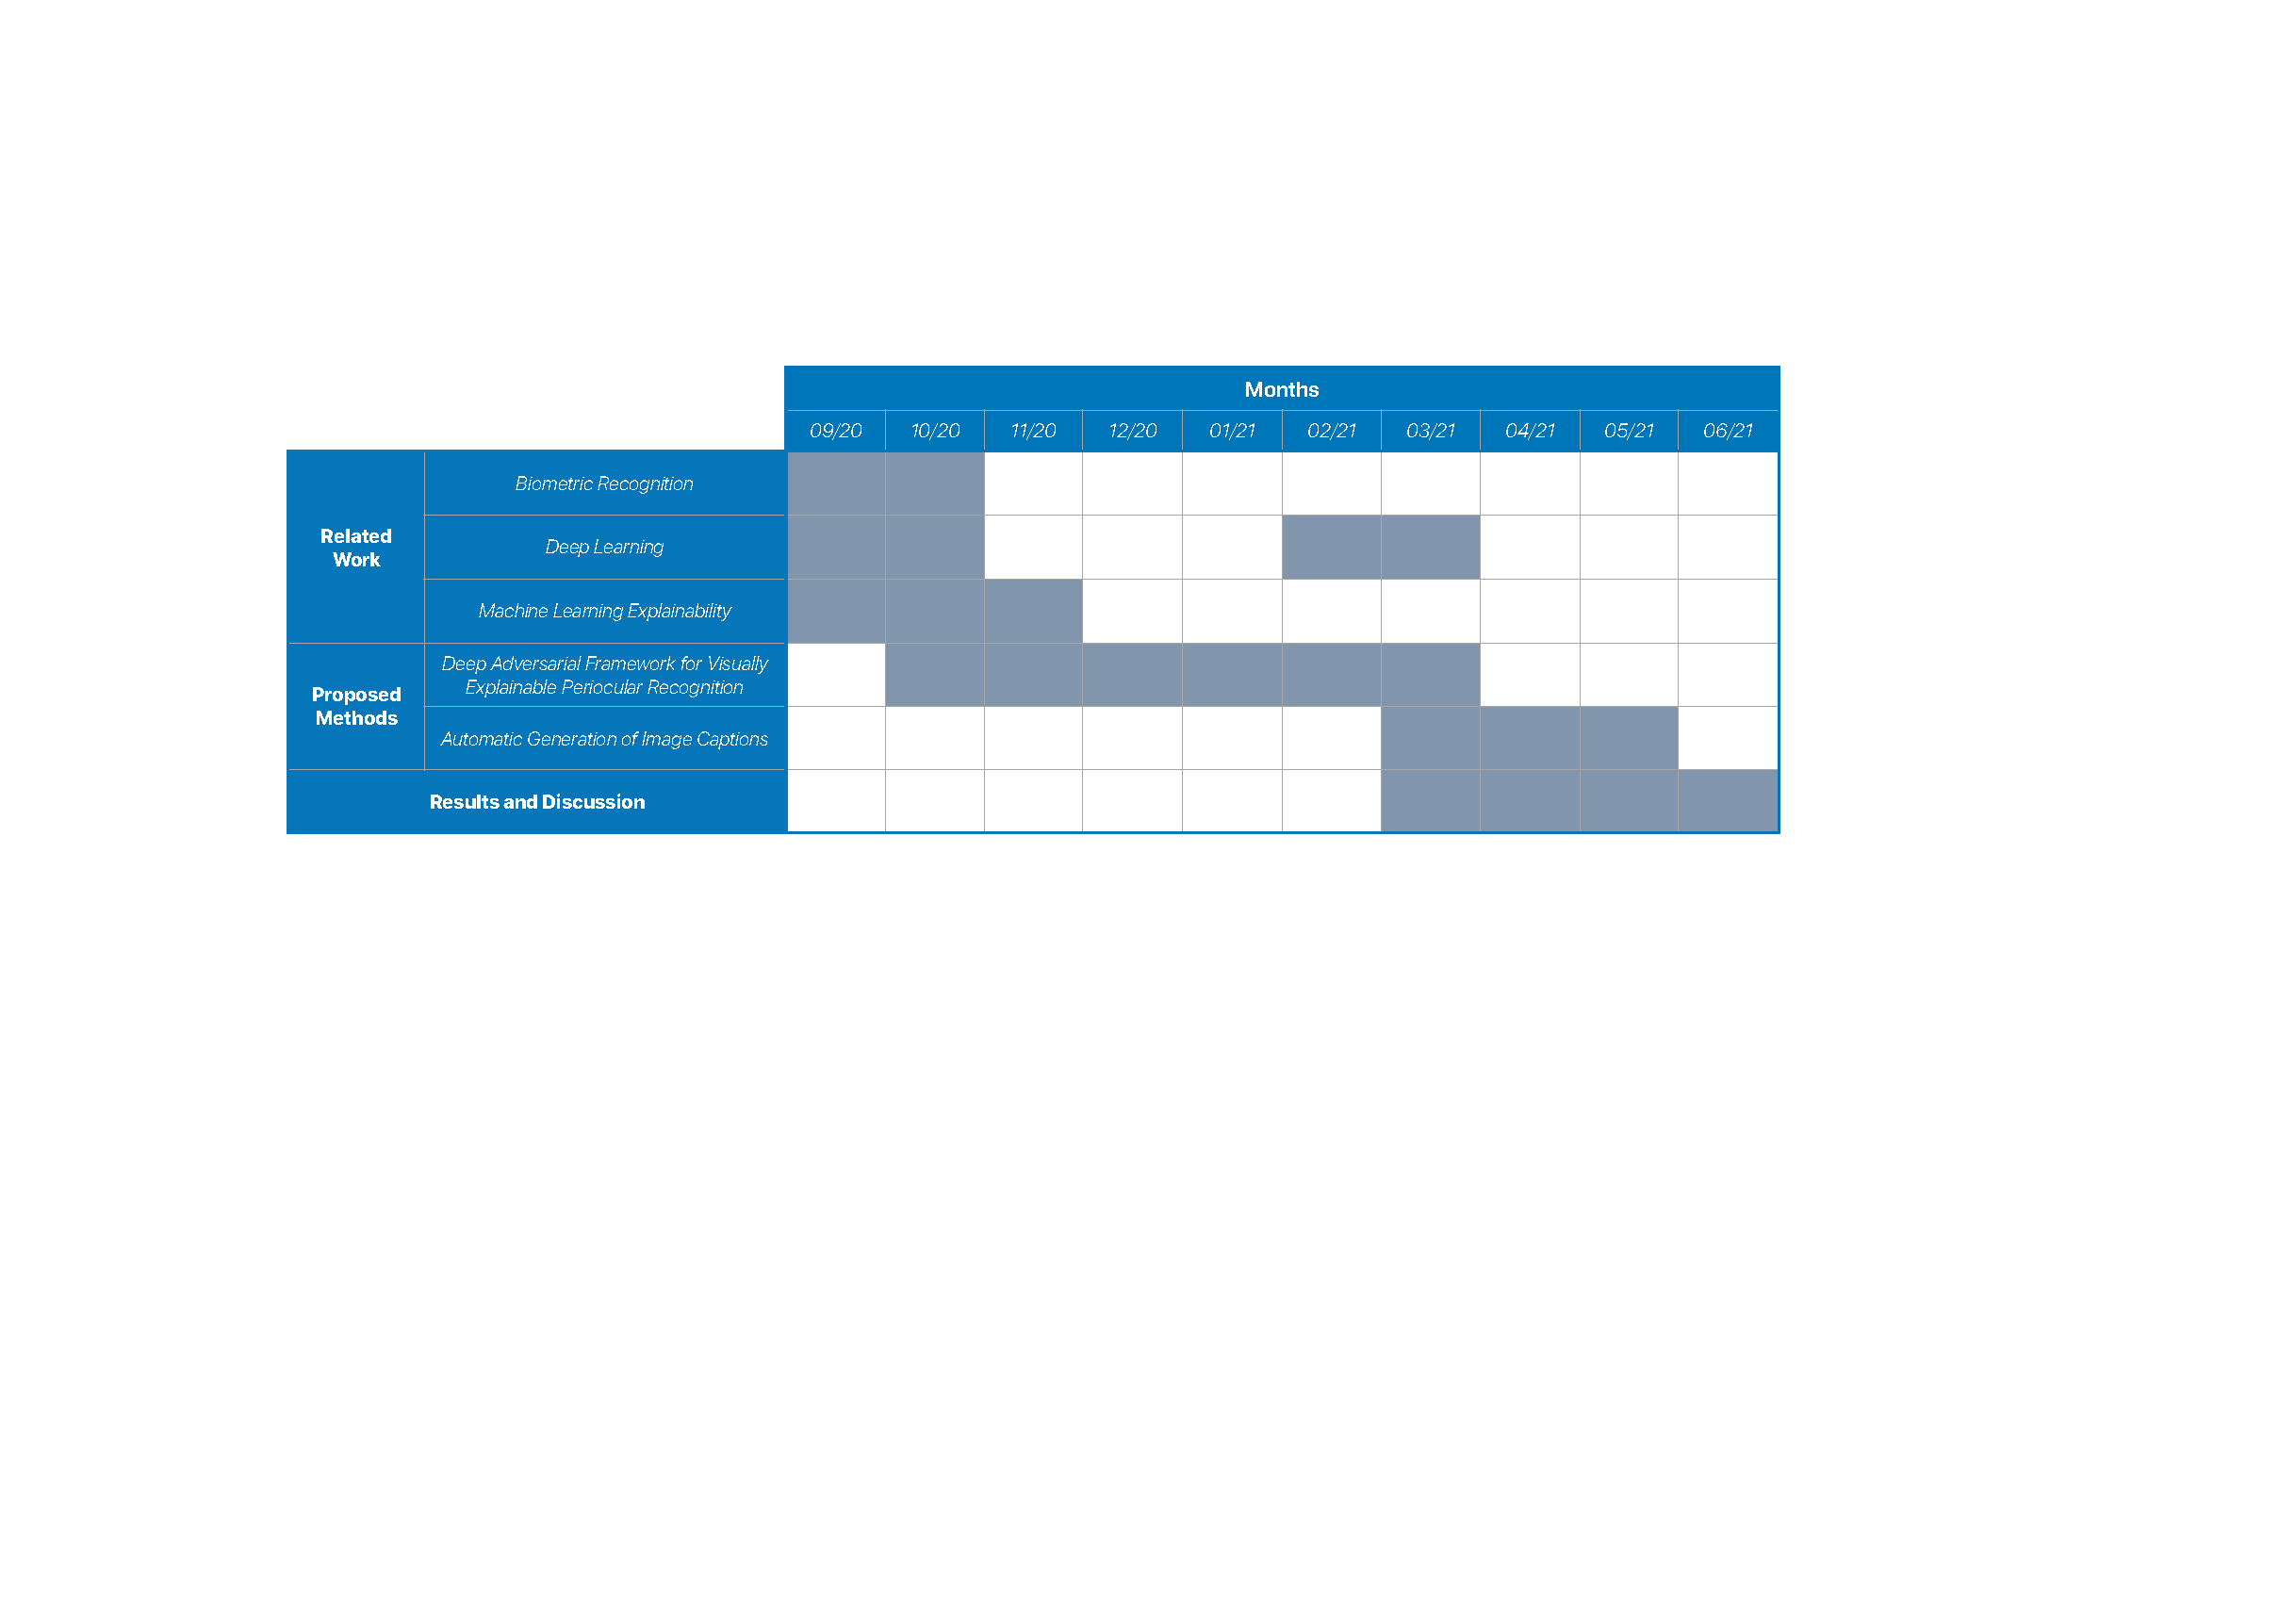
\includegraphics[width=405pt]{figures/figure_1.pdf}
\caption{Gantt diagram with the dissertation outline. With the exception of additional \ac{DL} research, the work went through a standard pipeline: research, development and testing.}
\label{fig:gantt_diagram}
\end{figure}